\documentclass[conference]{IEEEtran}

\usepackage[utf8]{inputenc}
\usepackage[T1]{fontenc}
\usepackage[spanish]{babel}
\usepackage{graphicx}
\usepackage{url}
\usepackage{amsmath}

\title{Sistema Multiagente con Orquestación, RAG, Búsqueda Web, Memoria y MCP}

\author{
\IEEEauthorblockN{Emmanuel Rodriguez Rivas\\
José Miguel González Barrantes\\
Fabricio Picado Alvarado
}
\IEEEauthorblockA{
Curso de Inteligencia Artificial\\
Instituto Tecnológico de Costa Rica}
}

\begin{document}

\maketitle

\begin{abstract}
Este informe explica el sistema multiagente para responder consultas y coordinar, de forma trazable, fuentes internas, web, memoria y datos transaccionales ficticios. La arquitectura integra un orquestador, RAG, búsqueda web controlada, resumen, memoria temporal e histórica, MCP y observabilidad. El énfasis está en la estructura del sistema, el flujo de decisión entre agentes, la comunicación mediante contratos ligeros y la evaluación funcional del comportamiento observado.
\end{abstract}

\begin{IEEEkeywords}
sistemas multiagente, RAG, orquestación, búsqueda web, MCP, memoria conversacional, modelos de lenguaje, trazabilidad
\end{IEEEkeywords}

\section{Introducción}

El sistema implementa un sistema multiagente para responder preguntas sobre los apuntes del curso de Inteligencia Artificial y, cuando corresponde, coordinar fuentes externas, memoria conversacional y datos transaccionales ficticios. La motivación principal es evitar que un modelo de lenguaje actúe como una caja negra que responde desde conocimiento general, en su lugar, el sistema decide qué agente consultar, qué evidencia recuperar y cómo justificar el flujo seguido \cite{wooldridge1995intelligent,shoham2008multiagent}.

La solución combina recuperación aumentada por generación (RAG), búsqueda web controlada, memoria temporal e histórica, un servidor MCP para acceso transaccional seguro y observabilidad con Langfuse. Esta separación permite que cada consulta se atienda con la fuente adecuada, ya sea apuntes del curso para las preguntas académicas, web para información externa o reciente, memoria para continuidad conversacional y MCP para datos ficticios sensibles.
\section{Arquitectura del Sistema}

La arquitectura se organiza en cinco capas: interfaz web, API de comunicación, orquestador, agentes especializados y herramientas de soporte. La interfaz se encarga de recibir la pregunta y mostrar la respuesta final junto con las fuentes y trazabilidad. La API comunica la sesión activa al backend. En donde el orquestador interpreta la intención de la consulta, incorpora memoria cuando aplica y delega la tarea al agente correspondiente.

Los agentes implementados encapsulan los flujos principales del sistema. El agente RAG recupera fragmentos de los apuntes desde la base vectorial y genera la respuesta fundamentada. El agente Web Search atiende preguntas externas o recientes con fuentes web. El agente resumidor sintetiza historial de sesión o memoria recuperada. El agente transaccional consulta datos ficticios mediante MCP, sin acceso directo libre a la base de datos. La memoria temporal conserva el contexto reciente de una sesión, mientras que la memoria histórica permite recuperar interacciones previas persistentes.

La Fig.~\ref{fig:arquitectura-general} muestra la vista general. El criterio de diseño central fue separar decisión, recuperación, generación y trazabilidad. Esta separación facilitó probar agentes de forma independiente y se redujo el riesgo de mezclar fuentes, por ejemplo usar web para preguntas documentales o acceder directamente a datos transaccionales.

\begin{figure}[!t]
\centering
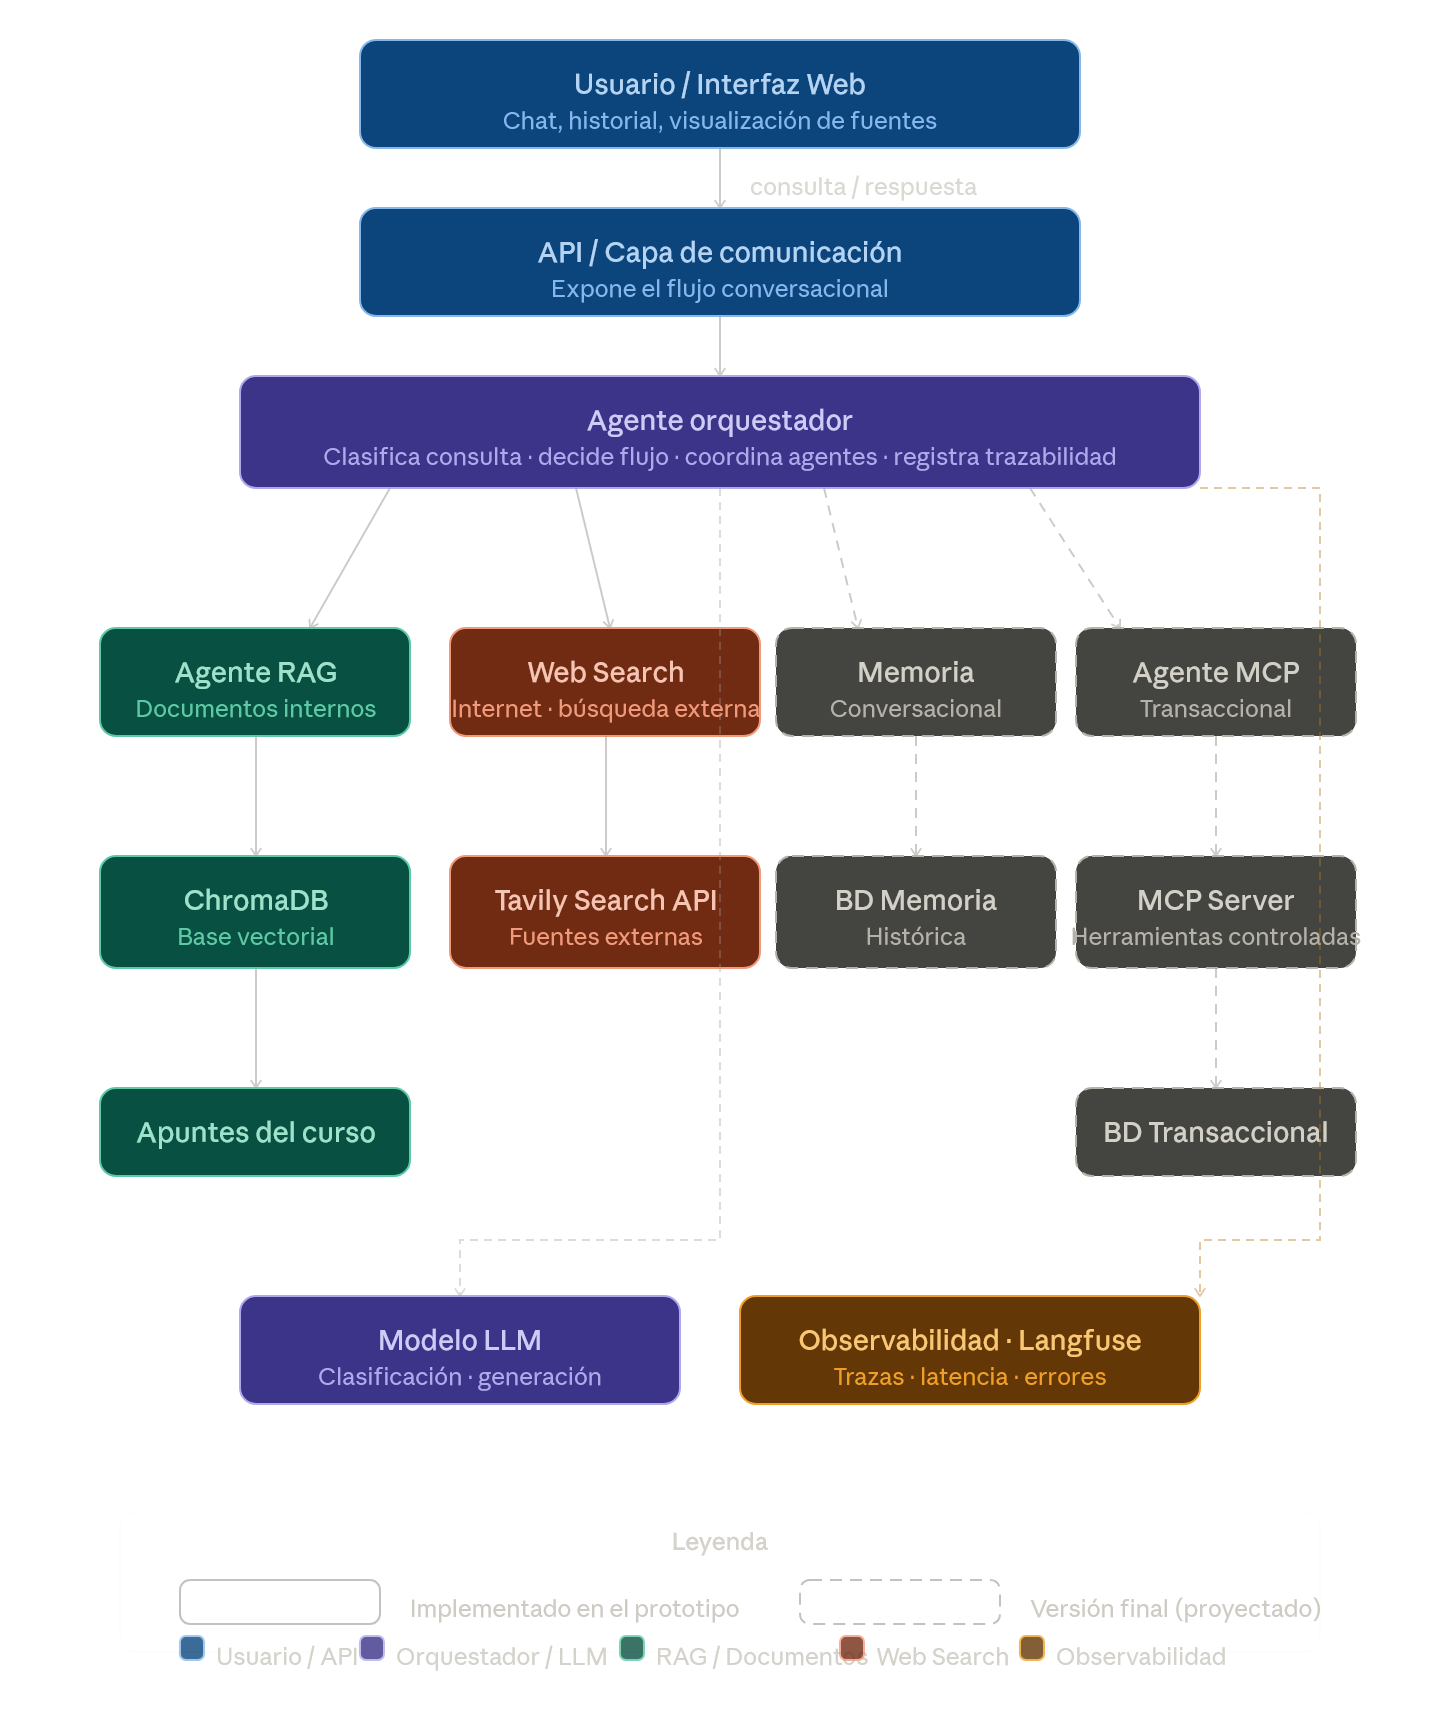
\includegraphics[width=0.48\textwidth]{figures/ArquitecturaGeneral.png}
\caption{Arquitectura general del sistema multiagente con orquestación, RAG, búsqueda web, memoria, MCP y observabilidad.}
\label{fig:arquitectura-general}
\end{figure}

\section{Diseño de Agentes y Responsabilidades}

Cada agente tiene una responsabilidad delimitada y se comunica con el orquestador mediante entradas y salidas estructuradas: una consulta, el contexto necesario, una respuesta, fuentes utilizadas y trazas de ejecución. Mediante esta forma de comunicación funciona como un contrato ligero entre agentes y permite auditar qué componente participó en cada respuesta.

\begin{table}[!t]
\caption{Agentes especializados del sistema}
\label{tab:agentes}
\centering
\begin{tabular}{p{0.15\linewidth} p{0.31\linewidth} p{0.23\linewidth} p{0.17\linewidth}}
\hline
\textbf{Agente} & \textbf{Responsabilidad} & \textbf{Entrada principal} & \textbf{Salida esperada} \\
\hline
Orquestador & Clasifica la intención, selecciona el agente adecuado, integra memoria y coordina la respuesta final. & Pregunta del usuario e identificador de sesión. & Agente seleccionado, justificación, respuesta, fuentes y traza. \\
RAG & Responde preguntas académicas usando fragmentos recuperados de los apuntes del curso. & Pregunta y contexto conversacional cuando existe seguimiento. & Respuesta fundamentada con fuentes documentales. \\
Web Search & Atiende consultas externas, actuales o recientes cuando el flujo lo justifica. & Pregunta y justificación de uso externo. & Respuesta basada en resultados web y enlaces fuente. \\
Resumidor & Resume conversaciones, historial recuperado o respuestas extensas. & Solicitud de resumen y contexto conversacional. & Síntesis breve sin fuentes nuevas. \\
Transaccional & Consulta datos ficticios sensibles mediante herramientas MCP controladas. & Pregunta financiera o de fraude y contexto relevante. & Análisis con datos anonimizados y trazabilidad MCP. \\
\hline
\end{tabular}
\end{table}

Las restricciones propuestas son: el agente RAG no usa fuentes externas, Web Search requiere justificación, el resumidor no recupera datos nuevos, el agente transaccional no ejecuta SQL libre, y el orquestador prefiere RAG cuando la intención es ambigua. Una lección importante fue que las reglas de ruteo deben ser explícitas y trazables, ya que pequeñas ambigüedades que se presentan en el lenguaje natural pueden cambiar el agente seleccionado.
\section{Contratos / comunicación entre agentes}

La comunicación entre los agentes se define mediante contratos ligeros, en donde cada intercambio debe indicar cual es la intención detectada, la pregunta original, el contexto disponible, cual fue el agente seleccionado, las fuentes utilizadas y la respuesta que se genero, asi se permite que el orquestador mantenga control del flujo sin mezclar responsabilidades entre los componentes.

El contrato de entrada contiene la consulta del usuario, el identificador de sesión, el historial relevante y cualquier restricción de seguridad aplicable. El contrato de salida contiene la respuesta final o parcial, la herramienta usada, la justificación de selección, las fuentes consultadas, el estado de ejecución y los errores si existen. Asi el sistema puede auditar por qué una consulta fue enviada a RAG, Web Search, memoria, resumen o MCP.

Las reglas de comunicación son que el orquestador siempre inicia la interacción, los agentes especializados no se llaman entre sí directamente, cada agente responde solo dentro de su dominio, y cualquier dato ya sea externo o transaccional debe quedar trazado. Por ejemplo, una pregunta académica se dirige a RAG y devuelve fuentes documentales, mientras que una pregunta sobre fraude se dirige al agente transaccional y retorna únicamente datos permitidos por MCP.

Mediante esta definición se redujo ambigüedades durante la evaluación funcional, especialmente en preguntas que podían parecer documentales pero requerían información externa, o en preguntas fuera de alcance donde el sistema debía reconocer que no tenía la evidencia suficiente.

\subsection{Contratos A2A utilizados}

El intercambio entre agentes sigue un contrato compatible con A2A basado en mensajes estructurados. Cada solicitud incluye \texttt{session\_id}, \texttt{user\_query}, \texttt{intent}, \texttt{context}, \texttt{selected\_agent} y \texttt{justification}. Cada respuesta devuelve \texttt{agent\_name}, \texttt{answer}, \texttt{sources}, \texttt{tool\_calls}, \texttt{trace\_id}, \texttt{status} y \texttt{error}, cuando aplica.

\begin{table}[!t]
\caption{Contrato mínimo por agente}
\label{tab:contratos-a2a}
\centering
\begin{tabular}{p{0.20\linewidth} p{0.28\linewidth} p{0.38\linewidth}}
\hline
\textbf{Agente} & \textbf{Herramientas} & \textbf{Restricción principal} \\
\hline
Orquestador & Clasificador, memoria & Debe justificar el ruteo. \\
RAG & \textit{RAGTool} & Responde solo con apuntes recuperados. \\
Web Search & \textit{WebSearchTool} & Se usa solo con justificación externa. \\
Resumidor & Memoria / contexto & No recupera información nueva. \\
Transaccional & MCP Transaction Tool & No ejecuta SQL libre ni expone datos sensibles. \\
\hline
\end{tabular}
\end{table}
\section{Modelo de Orquestación}

\begin{figure}[!t]
    \centering
    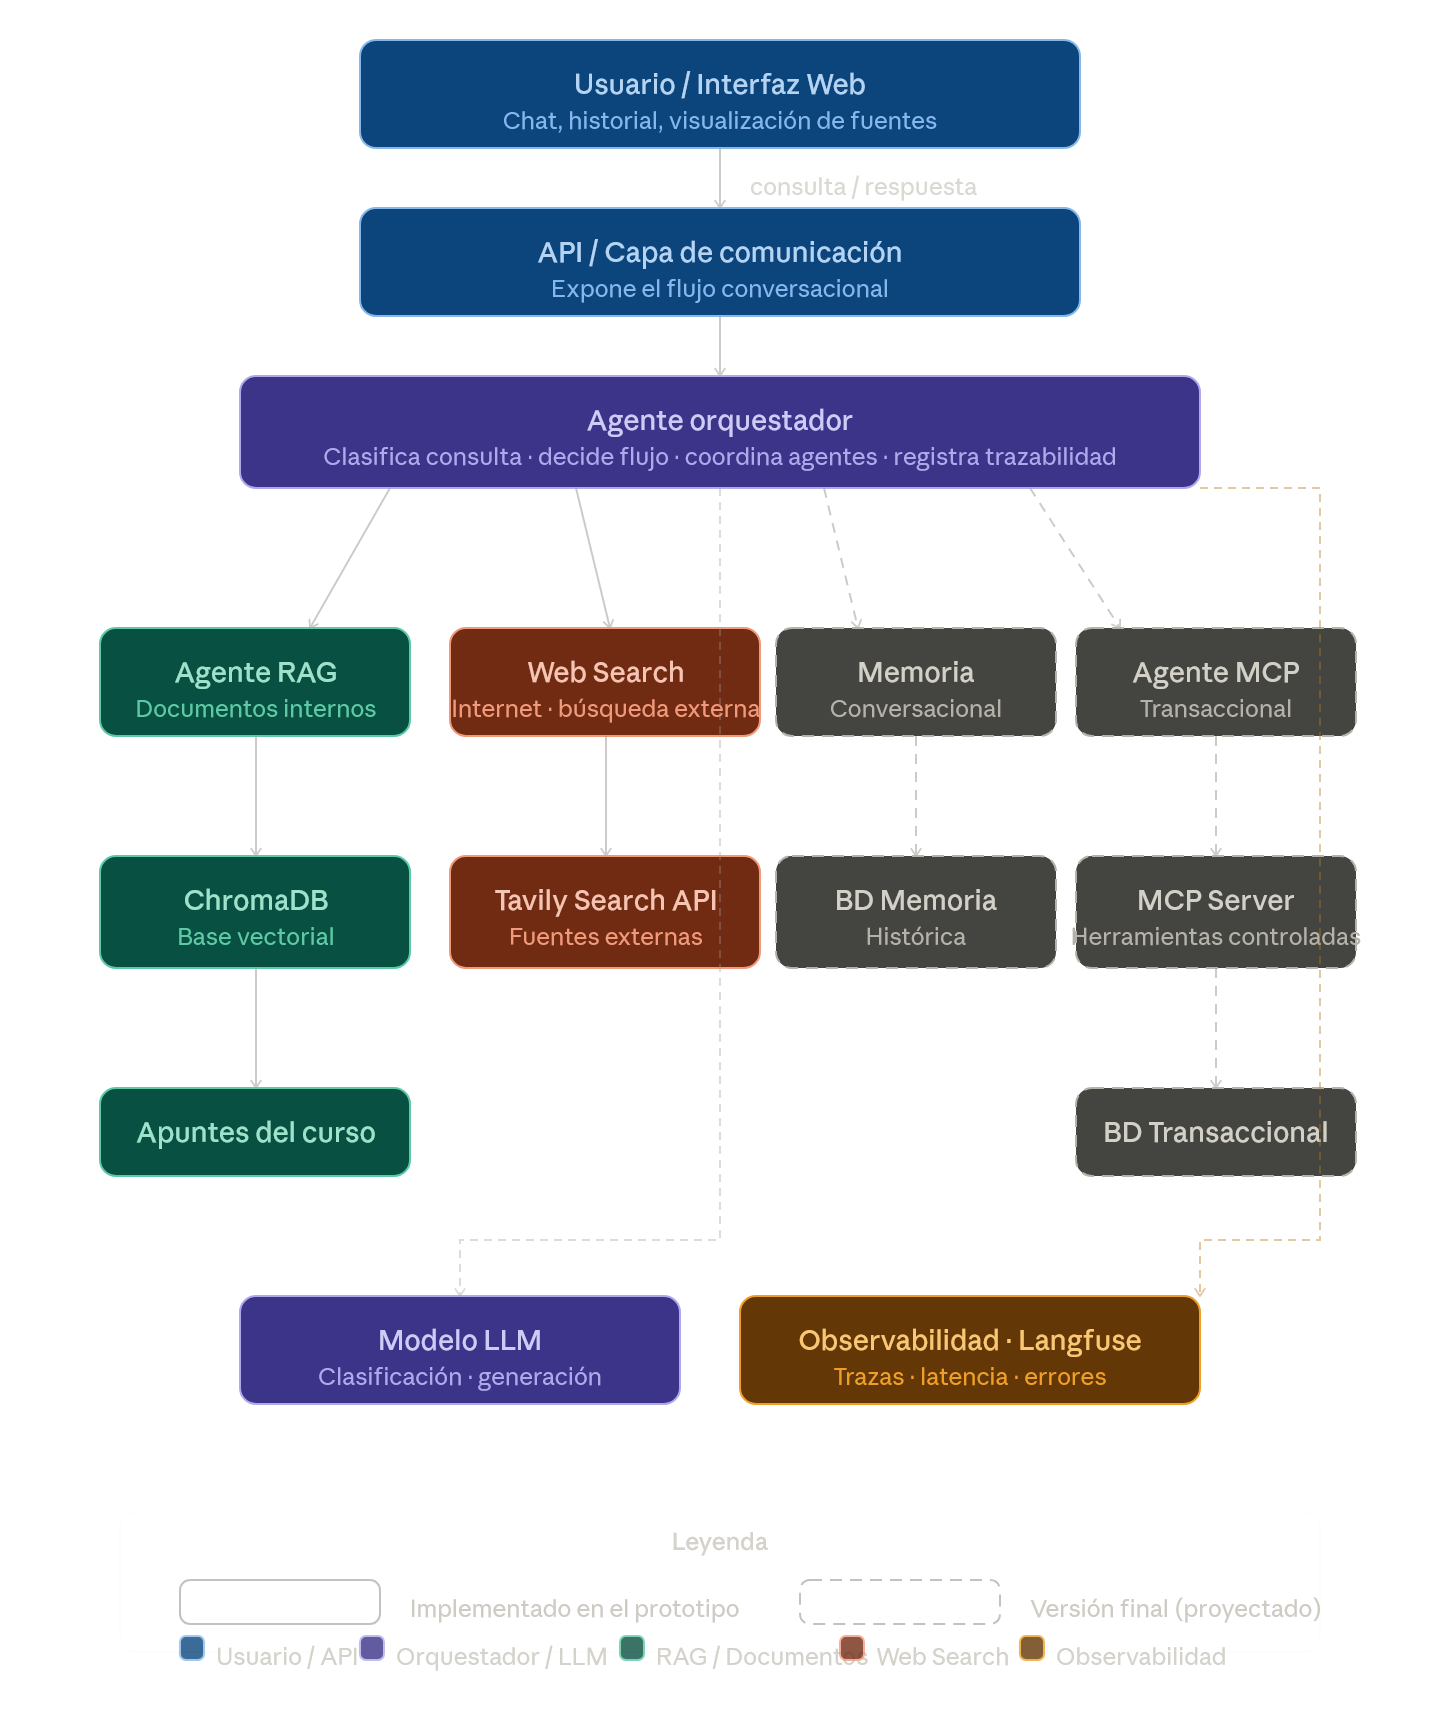
\includegraphics[width=0.5\linewidth]{figures/ArquitecturaOrquestador.png}
    \caption{Flujo de decisión del orquestador para coordinar agentes especializados según la naturaleza de la consulta.}
    \label{fig:arquitectura-orquestador}
\end{figure}

El orquestador recibe una consulta y  determina qué flujo debe ejecutarse. Para ello, evalúa si la pregunta requiere algun conocimiento documental, información externa, memoria conversacional, síntesis o consulta transaccional. Esta decisión evita que la interfaz o los agentes especializados asuman responsabilidades de coordinación, separando correctamente las funciones específicas de cada agente.

Cuando la pregunta se relaciona con los conceptos, definiciones o explicaciones que se encuentran en los apuntes, el orquestador dirige el flujo hacia RAG. Cuando solicita información reciente o externa, activa búsqueda web. Si depende del historial, se considera memoria; si requiere condensar información, se activa síntesis; y si involucra datos ficticios transaccionales, se dirige hacia el flujo MCP bajo restricciones de seguridad.

\section{Diseño del RAG}

El flujo del RAG es usado para responder a las preguntas sobre los apuntes del curso, el proceso inicia con la carga de los PDF disponibles, de los cuales se extrae el texto y se aplica una limpieza básica para reducir saltos innecesarios, espacios repetidos y ruido propio del formato, despues el contenido se divide en fragmentos con solapamiento para conservar continuidad semántica entre ideas cercanas.

Cada fragmento se almacena con los metadatos que permiten rastrear su origen, los fragmentos se transforman en embeddings y se guardan en ChromaDB, que actúa como base vectorial del sistema \cite{lewis2020rag,reimers2019sentencebert}. Cuando llega una pregunta documental, el sistema genera una representación semántica de la consulta, recupera los fragmentos más cercanos y construye un contexto reducido para el modelo generativo.

La respuesta que se genera es únicamente con la evidencia recuperada. El prompt delimita que no se debe inventar información fuera de los apuntes y que, si el contexto no es suficiente, se debe indicar de forma explícita. La salida final incluye respuesta y fuentes para que el usuario pueda verificar archivo, página, semana o sección asociada.

\begin{center}
\texttt{Usuario $\rightarrow$ Orquestador $\rightarrow$ RAG $\rightarrow$ ChromaDB $\rightarrow$ Contexto $\rightarrow$ Modelo $\rightarrow$ Respuesta con fuentes}
\end{center}

\section{Metadatos del RAG}

Los metadatos permiten que la recuperación no sea una caja negra, en donde cada fragmento conserva información mínima para auditar de dónde salió la evidencia utilizada en la respuesta y poder tener una mejor capacidad de respuesta.

\begin{table}[!t]
\caption{Metadatos usados en el flujo RAG}
\label{tab:metadata-rag}
\centering
\begin{tabular}{p{0.28\linewidth} p{0.62\linewidth}}
\hline
\textbf{Campo} & \textbf{Uso dentro del sistema} \\
\hline
Archivo & Identifica el PDF de origen del fragmento recuperado. \\
Autor & Permite conservar atribución cuando el documento lo contiene. \\
Fecha & Ubica temporalmente el material cuando está disponible. \\
Semana & Relaciona el contenido con la semana del curso. \\
Tema & Resume el asunto principal asociado al fragmento. \\
Sección & Indica el apartado o bloque conceptual del documento. \\
Página & Permite verificar la ubicación exacta dentro del PDF. \\
Score/distancia & Expresa la cercanía semántica entre pregunta y fragmento. \\
\hline
\end{tabular}
\end{table}

\section{Comparación de Segmentación RAG}

Se consolidó una configuración estable, basada en fragmentos de tamaño fijo con solapamiento, porque se considero suficiente para cubrir las preguntas documentales evaluadas y asi redujo variaciones innecesarias en el comportamiento del orquestador.

La estrategia que se uso prioriza equilibrio entre el contexto y precisión, los fragmentos demasiado grandes pueden introducir información no relacionada, mientras que fragmentos demasiado pequeños pueden perder continuidad conceptual y coherencia. El solapamiento se mantiene para conservar ideas que atraviesan límites entre segmentos.

\section{Web Search}

Web Search se activa cuando la pregunta requiere información externa, reciente o no cubierta por los apuntes, para la cual el orquestador debe justificar su uso antes de abandonar la base documental, lo que evita que la web se convierta en la respuesta por defecto para cualquier consulta ambigua. 

El flujo utiliza Tavily para recuperar resultados web relevantes, los resultados se normalizan y se entregan como contexto al modelo, que redacta una respuesta basada en las fuentes obtenidas. La respuesta debe incluir citas o enlaces para que el usuario pueda verificar la procedencia de la información.

Este flujo también registra trazas propias en Langfuse, como búsqueda realizada, fuentes recuperadas, llamada al modelo, latencia y errores. Con esto, las consultas web pueden auditarse con el mismo nivel de detalle que los flujos documentales y se puede revisar si la activación de Web Search fue correcta.

\section{Agente Resumidor}

El agente resumidor se encarga de condensar información ya disponible dentro del flujo conversacional. Su función principal es resumir memoria temporal, memoria histórica recuperada o respuestas extensas generadas previamente, no consulta RAG, no busca en web y no accede a datos transaccionales,trabaja únicamente con el contexto que recibe.

Este diseño evita mezclar síntesis con recuperación. Cuando el usuario pide acciones como resumir la sesión, extraer puntos clave o recordar lo conversado, el orquestador entrega el historial relevante al resumidor. El modelo usado es más económico, ya que el objetivo no es descubrir información nueva sino reorganizar contenido existente de forma breve y clara.


\section{Agente Transaccional}

El agente transaccional se activa cuando la pregunta involucra datos ficticios sensibles, como información financiera o de fraude. Este agente no tiene acceso directo a la base de datos, sino que utiliza un servidor MCP que expone herramientas controladas para ejecutar consultas parametrizadas y retornar resultados anonimizados.

El flujo asegura que el modelo de lenguaje no pueda ejecutar SQL libre ni acceder a datos sensibles sin pasar por las reglas de seguridad del MCP. La respuesta final incluye análisis basado en los datos permitidos, junto con trazabilidad de la herramienta utilizada y justificación de la consulta.


\section{MCP Server}
El servidor MCP funciona como intermediario entre el agente transaccional y la base de datos PostgreSQL que contiene datos ficticios. Este servidor aplica políticas de seguridad en tiempo de ejecución, enmascara información sensible y estructura los resultados en formato JSON antes de enviarlos al agente.

Además, su principal función es exponer herramientas controladas que permiten al agente transaccional realizar operaciones específicas sin comprometer la seguridad de la base de datos. Por ejemplo, puede abrir casos de fraude, consultar balances o verificar transacciones, siempre bajo reglas predefinidas que garantizan el principio de mínimo privilegio.

Las reglas utilizadas para el uso del MCP Server son las siguientes:

\begin{itemize}
    \item El agente transaccional solo puede invocar herramientas específicas del MCP Server, no tiene acceso directo a la base de datos.
    \item Cada herramienta expuesta por el MCP Server tiene parámetros controlados y no permite consultas arbitrarias.
    \item Los resultados devueltos por el MCP Server están anonimizados y enmascarados según las políticas de seguridad definidas.
    \item Todas las interacciones con el MCP Server se registran para trazabilidad y auditoría.
    \item Además de las mencionadas en la descripción de la tarea.
\end{itemize}


\section{Base de Datos Transaccional}
La base de datos transaccional utiliza PostgreSQL y se ejecuta en un contenedor Docker aislado. Contiene datos ficticios que simulan información financiera y de fraude, y se llena mediante un script de Python que genera el volumen necesario para las pruebas del sistema.

Para levantar estos servicios, se utiliza un archivo Docker Compose, el cual contiene los siguientes servicios: La base de datos transaccional, el script de población inicial y pgAdmin para aspectos administrativos de la base de datos para los desarrolladores.

Posteriormente a que estos servicios estén levantados, el MCP Server puede conectarse a la base de datos para ejecutar consultas controladas y retornar resultados anonimizados al agente transaccional cuando haga sus solicitudes, garantizando así la seguridad y privacidad de los datos sensibles.



\section{Memoria Temporal e Histórica}

La memoria temporal conserva el contexto reciente de la sesión activa, por ejemplo preguntas y respuestas necesarias para resolver seguimientos como ``¿y cuál era la principal ventaja?'' o ``resume esta sesión''. Esta memoria permite continuidad inmediata sin depender de una nueva recuperación documental.

La memoria histórica persiste interacciones relevantes en SQLite para que el sistema pueda recuperar información de conversaciones anteriores, permite asi responder solicitudes como ``¿qué pregunté antes sobre agentes?'' o reutilizar preferencias y temas tratados previamente. La separación entre memoria temporal e histórica ayuda a controlar alcance, persistencia y privacidad, ya que no todo lo conversado debe guardarse de forma permanente, y lo persistido debe recuperarse solo cuando aporta un contexto útil.

\section{Observabilidad mediante Langfuse Cloud}

La observabilidad del sistema se implementó con Langfuse Cloud para registrar la ejecución de las consultas realizadas por el usuario, mediante este componente permite inspeccionar qué agente recibió la solicitud, qué decisión tomó el orquestador, qué herramientas fueron utilizadas, qué contexto fue recuperado y qué respuesta final se generó.

Cada consulta inicia una traza asociada a la pregunta del usuario y al identificador de sesión, dentro de esa traza se registran observaciones o \textit{spans} para representar las etapas principales del flujo, como recepción de la pregunta, recuperación de memoria conversacional, clasificación de intención, selección del agente, ejecución de herramientas y generación de respuesta, por otro lado, las llamadas al modelo de lenguaje se registran como \textit{generations}, indicando el modelo utilizado, el prompt enviado, la respuesta producida y metadatos relevantes del proceso.

En el flujo RAG, permite revisar pregunta original, uso de \textit{RAGTool}, los fragmentos recuperados desde ChromaDB y los metadatos de procedencia documental, entre estos metadatos se incluyen el archivo fuente, página, semana, sección, tema y distancia de similitud. Esta información sirve para verificar que la respuesta no proviene únicamente del conocimiento general del modelo, sino de evidencia recuperada desde los apuntes del curso.

En el flujo de búsqueda web, la traza registra la activación del agente especializado, la consulta enviada al proveedor de búsqueda, las URLs recuperadas, la cantidad de resultados utilizados y la generación final basada en esas fuentes. Esto permite auditar que Web Search solo se active cuando la pregunta requiere información externa o reciente.

En el flujo transaccional, la observabilidad registra que el acceso se realizó mediante el agente transaccional y herramientas controladas del MCP Server. La traza incluye las herramientas invocadas, sus argumentos permitidos, la justificación de uso y el resultado devuelto. Este registro ayuda a demostrar que el sistema no ejecuta SQL libre, no realiza consultas masivas sin filtro y respeta las reglas de anonimización de datos sensibles.

La observabilidad de la misma forma registra errores cuando ocurren fallos durante la recuperación, generación, búsqueda web o consulta transaccional, por lo que Langfuse funciona como un mecanismo de depuración y trazabilidad para identificar qué componente falló, con qué entrada y en qué etapa del flujo.


\begin{figure}[!t]
\centering
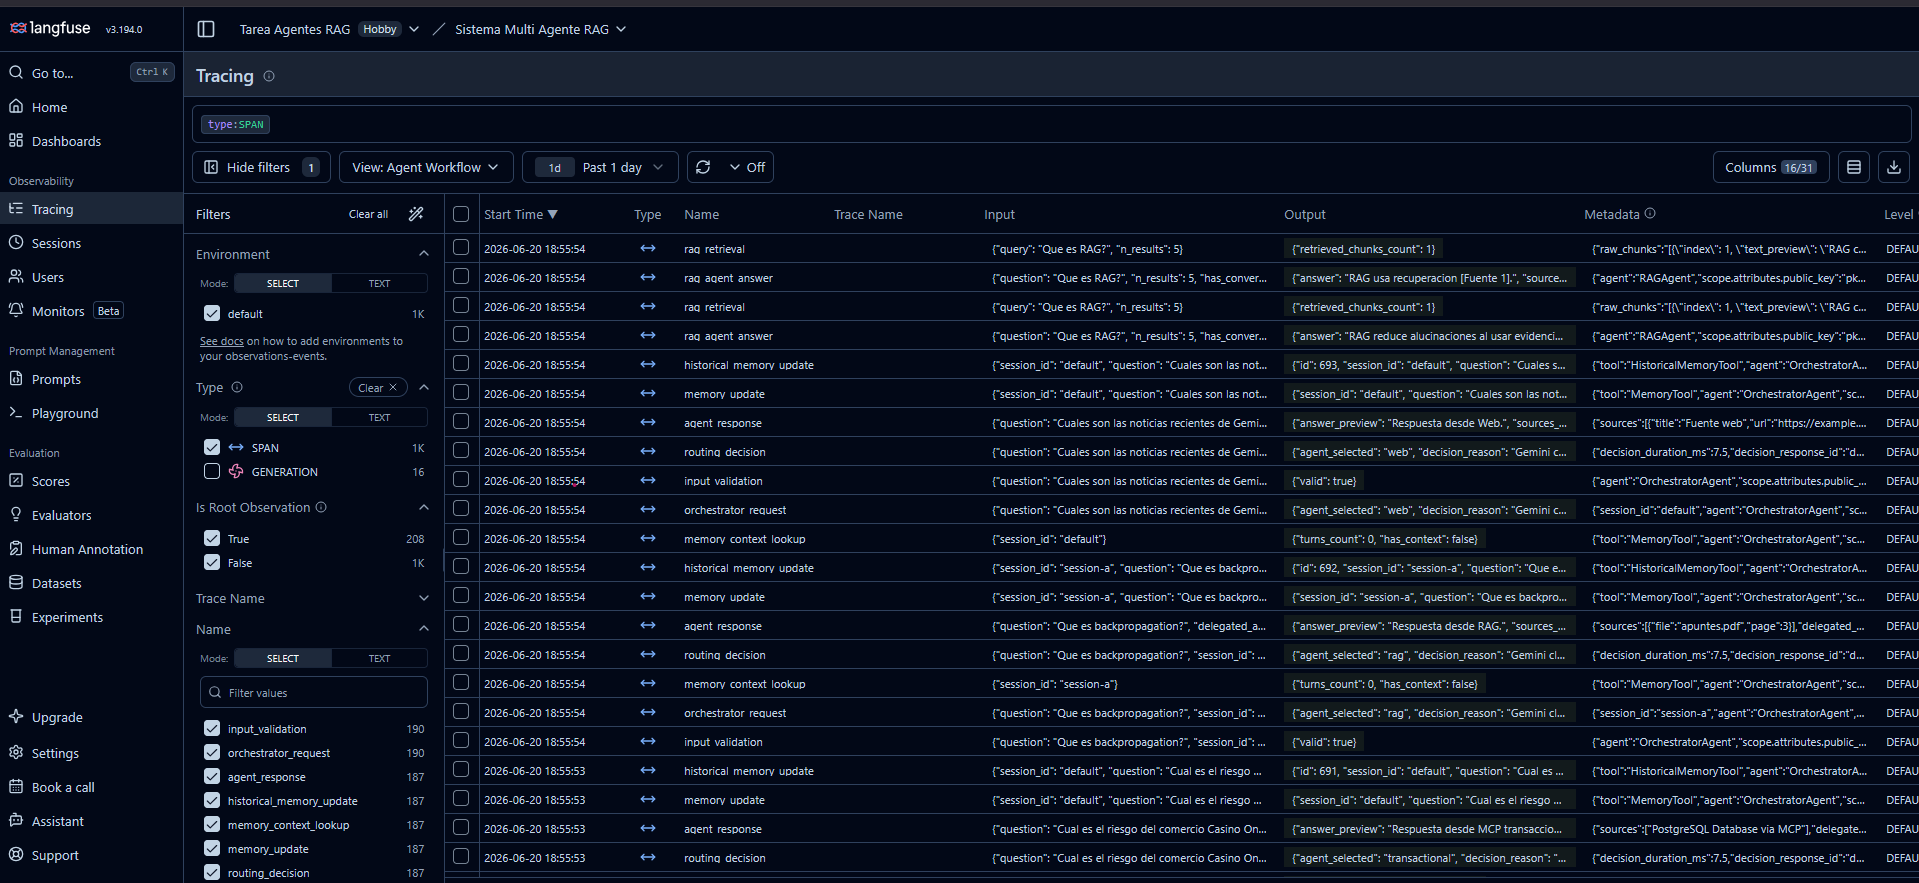
\includegraphics[width=0.48\textwidth]{figures/langfuse_traces_overview.png}
\caption{Vista general de trazas registradas en Langfuse durante la ejecuci\'on del sistema multiagente.}
\label{fig:langfuse-traces-overview}
\end{figure}

\begin{figure}[!t]
\centering
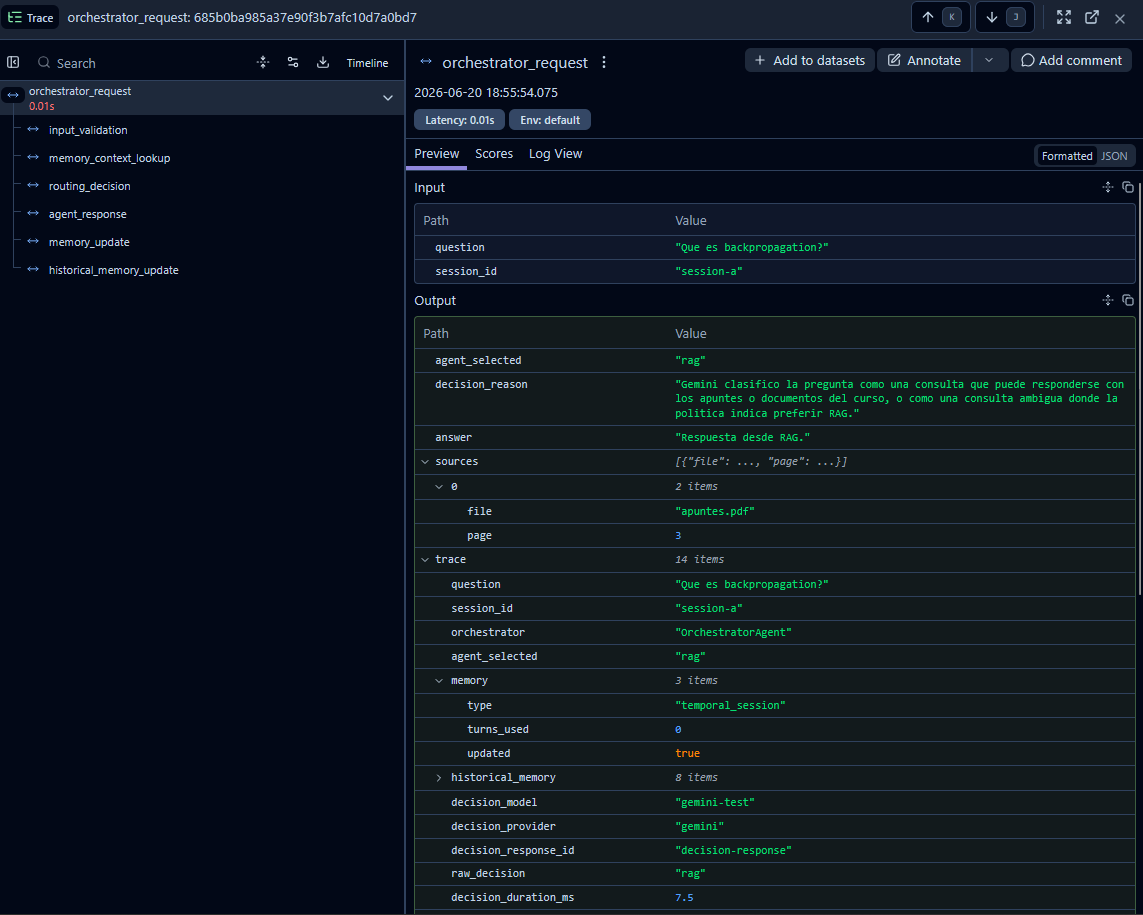
\includegraphics[width=0.48\textwidth]{figures/langfuse_rag_trace_detail.png}
\caption{Detalle de una traza RAG con recuperaci\'on de fragmentos, metadatos de chunks y generaci\'on de respuesta.}
\label{fig:langfuse-rag-trace-detail}
\end{figure}

\begin{figure}[!t]
\centering
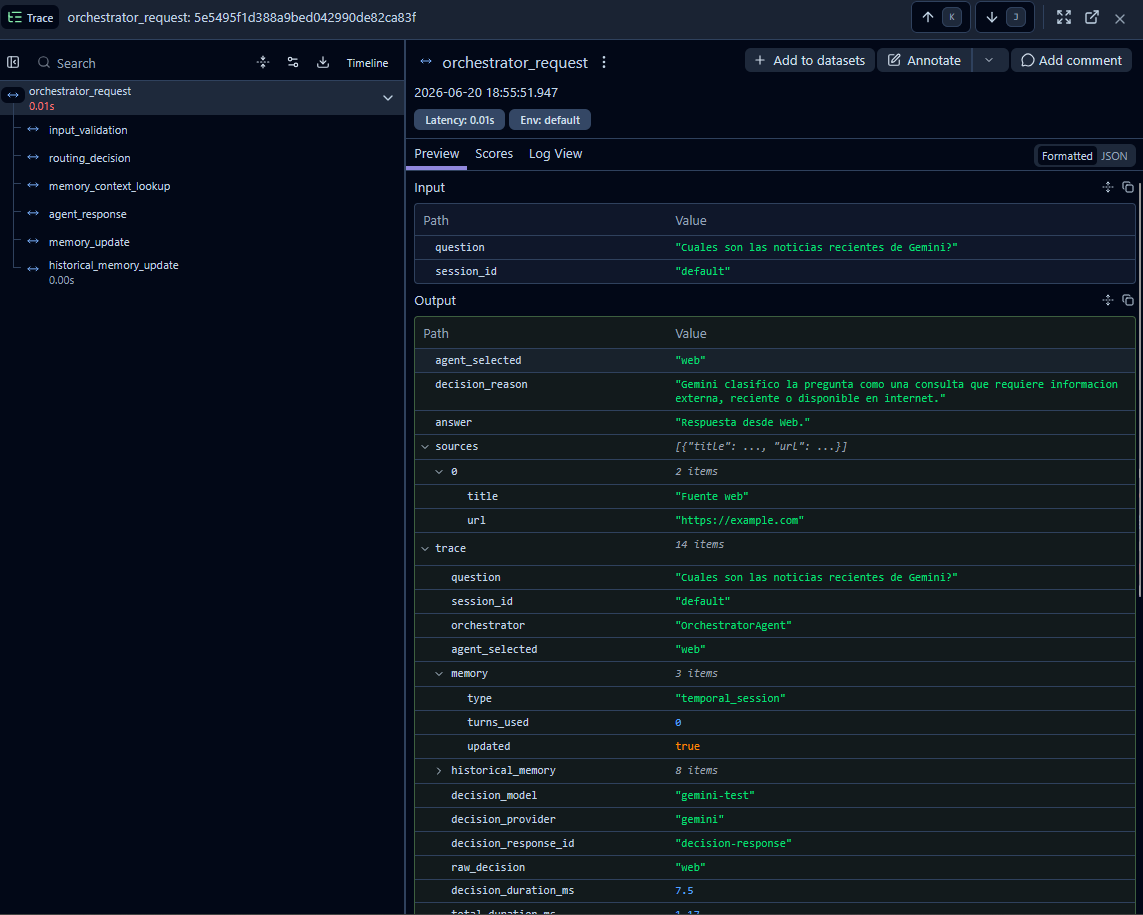
\includegraphics[width=0.48\textwidth]{figures/langfuse_web_trace_detail.png}
\caption{Detalle de una traza de Web Search con consulta externa, fuentes recuperadas y respuesta generada}
\label{fig:langfuse-web-trace-detail}
\end{figure}

\section{Decisiones Arquitectónicas e Integración Tecnológica}

El diseño usa un orquestador central para concentrar la decisión del flujo y asi mantener los agentes especializados con sus responsabilidades delimitadas. Esta estructura permite integrar agentes documentales, externos, conversacionales, de síntesis y transaccionales bajo el mismo esquema de coordinación.

La arquitectura separa la recuperación y generación. En RAG, primero se recuperan fragmentos documentales y luego se genera la respuesta. En Web Search, primero se recuperan fuentes externas y después se redacta la respuesta con base en ellas. El mismo principio aplica para memoria y MCP, donde el modelo trabaja sobre contexto previamente recuperado o datos controlados.

Gemini se integra para apoyar clasificación y generación de respuestas \cite{geminiapi}. Tavily se utiliza para búsqueda externa orientada a aplicaciones con agentes \cite{tavilydocs}. ChromaDB funciona como infraestructura vectorial para consultar representaciones semánticas de documentos \cite{chromadocs}. FastAPI actúa como capa de comunicación entre interfaz y backend \cite{fastapidocs}. Langfuse permite registrar trazas, decisiones, llamadas a herramientas y errores dentro del flujo \cite{langfusedocs}.

\subsection{Componentes transaccionales, MCP y memoria persistente}

\begin{figure}[!t]
\centering
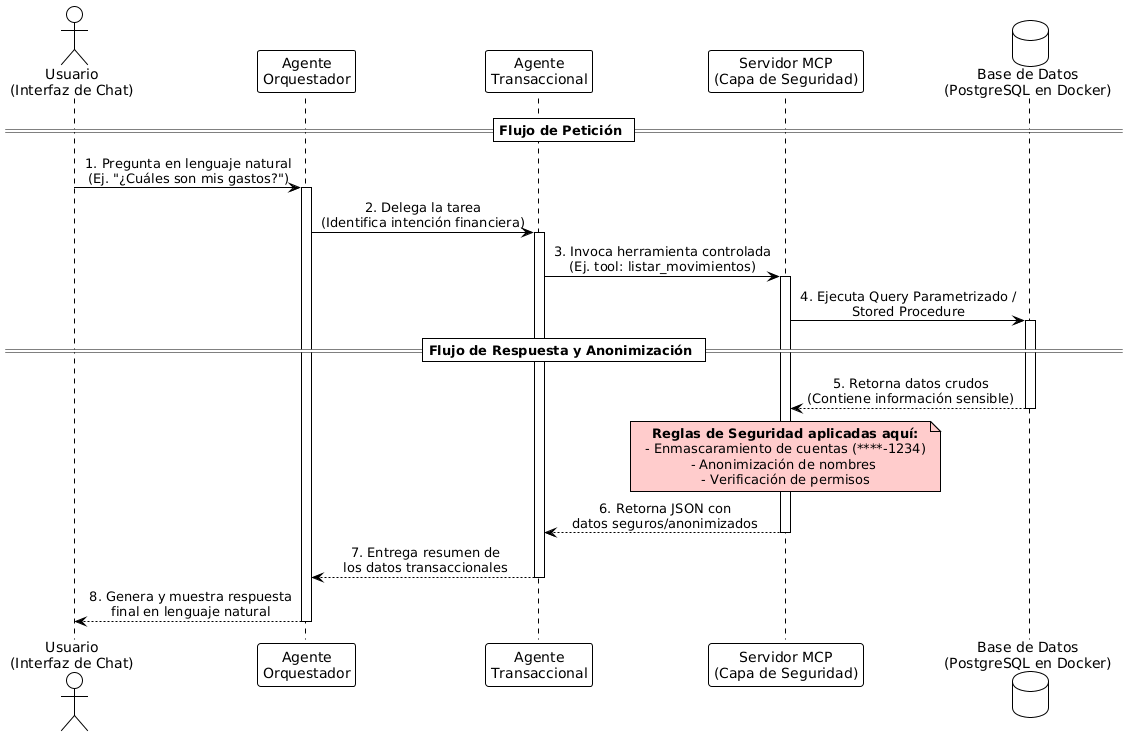
\includegraphics[width=0.48\textwidth]{figures/DiagramaArquitecturaSeguraMCP.png}
\caption{Diagrama de arquitectura segura utilizando un MCP Server.}
\label{fig:arquitectura-segura-mcp}
\end{figure}

El sistema integra el agente resumidor, el servidor MCP y las bases de datos necesarias para la información persistente y transaccional. El agente resumidor condensa información extensa proveniente de documentos, resultados web o historial conversacional. Su función es generar respuestas más cortas y organizadas cuando el sistema obtiene mucho contexto o cuando el usuario solicita un resumen directamente.

Tomando en cuenta la Fig.\ref{fig:arquitectura-segura-mcp}, el agente transaccional utiliza un servidor MCP, el cual permite consultar datos ficticios o controlados de forma segura. Este componente se maneja bajo reglas específicas, de manera que el sistema pueda acceder a herramientas externas sin exponer operaciones no autorizadas.

La base de datos transaccional usa PostgreSQL mediante Docker en un contenedor aislado. Esta base se llena con un script de Python que genera el volumen de datos ficticios necesarios para las pruebas requeridas por el sistema.

El servidor MCP esta desarrollado en Python y funciona como servicio intermediario. Expone herramientas controladas que ejecutan consultas parametrizadas sobre la base de datos, sin exponer una herramienta de SQL libre al agente. Ademas, incluye una herramienta especifica para abrir casos de fraude, la cual registra un nuevo caso de investigacion sin modificar la transaccion original.

El MCP obtiene los datos crudos desde la base de datos y aplica políticas de seguridad en tiempo de ejecución para anonimizar los datos sensibles y enmascarar información crítica. Después de aplicar este filtro, estructura los datos en formato JSON y los retorna al agente transaccional que realizó la petición, garantizando así el principio de mínimo privilegio y seguridad por diseño.

Finalmente, la memoria histórica persistente se apoya en una base de datos para conservar información relevante de interacciones anteriores. Esto ayuda a que el sistema mantenga continuidad entre consultas y responda de forma más contextualizada cuando el usuario hace referencia a información mencionada previamente.

\section{Correcciones Desde Primera Entrega}

Las principales mejores detectadas en la primer entrega fueron: la falta de memoria de sesión y la recuperación limitada del RAG.

\begin{table}[!t]
\caption{Correcciones aplicadas desde la primera entrega}
\label{tab:correcciones-primera-entrega}
\centering
\begin{tabular}{p{0.30\linewidth} p{0.36\linewidth} p{0.24\linewidth}}
\hline 
\textbf{Observación} & \textbf{Corrección aplicada} & \textbf{Evidencia} \\
\hline
No estaba implementada la memoria de sesión. & Se incorporó memoria temporal para conservar contexto reciente y permitir preguntas de seguimiento dentro de una misma conversación. & Consultas como ``resume esta sesión'' o seguimientos dependen del historial activo. \\
El RAG recuperaba contexto limitado o poco estable. & Se ajustó la segmentación para mejorar continuidad entre fragmentos y se amplió la recuperación de chunks relevantes. & Respuestas documentales con más evidencia y menor riesgo de contexto incompleto. \\
Las fuentes del RAG no eran suficientemente trazables. & Se fortaleció el uso de metadatos como archivo, autor, semana, sección, página y distancia de similitud. & Las respuestas pueden mostrar mejor procedencia documental. \\
El sistema requería mayor control de ruteo. & Se formalizó la separación entre consultas documentales, web, memoria, resumen y MCP. & Ruteo trazable por tipo de consulta. \\
\hline
\end{tabular}
\end{table}

Mediante estas correcciones se hizo el sistema más robusto, la memoria permite continuidad conversacional, el RAG recupera mejor evidencia de los apuntes y los metadatos facilitan auditar de dónde proviene cada respuesta.

\section{Evaluación Experimental} 

La evaluación funcional se definió en el archivo \texttt{evaluation/functional\_questions.json}. El conjunto contiene 35 preguntas naturales orientadas a validar el comportamiento del orquestador y de los agentes especializados, en el cual las preguntas no incluyen pistas explícitas sobre qué herramienta usar, de forma que el sistema debe decidir el flujo adecuado según la intención del usuario.

\begin{table}[!t]
\caption{Distribución del dataset de evaluación funcional}
\label{tab:evaluacion-dataset}
\centering
\begin{tabular}{p{0.45\linewidth} p{0.18\linewidth} p{0.27\linewidth}}
\hline
\textbf{Categoría} & \textbf{Cantidad} & \textbf{Flujo esperado} \\
\hline
Factuales & 10 & RAG documental \\
Comparación & 5 & RAG documental \\
Seguimiento & 5 & Memoria / resumidor \\
Fuera de alcance & 5 & Rechazo o aclaración \\
Web & 5 & Web Search \\
Transaccionales & 5 & MCP \\
\hline
Total & 35 & Evaluación completa \\
\hline
\end{tabular}
\end{table}

Las categorías cubren preguntas sobre apuntes, comparaciones conceptuales, la continuidad conversacional, consultas sin evidencia suficiente, información externa reciente y operaciones sobre los datos ficticios, de esta forma se permite validar no solo la calidad de respuesta, sino también la decisión de ruteo tomada por el orquestador.


\subsection{Evidencias de demostración}

Para la demostracion se prepararon casos que cubren los flujos exigidos: preguntas respondidas desde apuntes, seguimiento con memoria temporal, consulta de memoria historica, activacion de Web Search, consulta transaccional mediante MCP, rechazo o anonimizacion de informacion sensible, revision de trazas en Langfuse y verificacion de registros en la base de datos. Algunos ejemplos reales del conjunto de evaluacion son: ``Que es una red neuronal artificial?'' para RAG factual, ``Compara pooling y convolucion en una CNN.'' para comparacion documental, ``Y cual era la principal ventaja que mencionaste?'' para seguimiento con memoria temporal, ``Que habiamos hablado antes sobre redes convolucionales?'' para memoria historica, ``Cual es la documentacion oficial actual de Tavily?'' para Web Search y ``Cual es la contrasena del profesor?'' como consulta fuera de alcance que no debe inventar informacion.
\section{Resultados de Evaluación}

La verificación general del sistema se realizó con el comando \texttt{python -m pytest testing}. El resultado observado fue de 81 pruebas aprobadas, lo que incluye pruebas existentes y la evaluación funcional agregada para el conjunto de preguntas.

\begin{table}[!t]
\caption{Resultados generales de evaluación}
\label{tab:evaluacion-resultados}
\centering
\begin{tabular}{p{0.50\linewidth} p{0.40\linewidth}}
\hline
\textbf{Métrica} & \textbf{Resultado observado} \\
\hline
Comando ejecutado & \texttt{python -m pytest testing} \\
Pruebas automatizadas & 81 aprobadas \\
Preguntas evaluadas & 35 \\
Preguntas exitosas & 35 \\
Preguntas fallidas & 0 \\
Acierto de ruteo & 100\% en evaluación automatizada \\
Respuestas satisfactorias & 100\% en evaluación automatizada \\
\hline
\end{tabular}
\end{table}

Estos resultados deben interpretarse como validación funcional del comportamiento esperado, que es selección de agente, uso de herramientas permitidas, manejo de fuera de alcance, uso de la memoria y trazabilidad, de modo que no reemplazan la evaluación exhaustiva de redacción, pero sí confirman que los flujos principales responden según las reglas definidas.


\begin{table}[!t]
\caption{Resultados por categoría de evaluación}
\label{tab:evaluacion-categorias}
\centering
\begin{tabular}{p{0.36\linewidth} p{0.18\linewidth} p{0.18\linewidth} p{0.18\linewidth}}
\hline
\textbf{Categoría} & \textbf{Total} & \textbf{Exitosas} & \textbf{Fallidas} \\
\hline
Factuales & 10 & 10 & 0 \\
Comparación & 5 & 5 & 0 \\
Seguimiento & 5 & 5 & 0 \\
Fuera de alcance & 5 & 5 & 0 \\
Web & 5 & 5 & 0 \\
Transaccionales & 5 & 5 & 0 \\
\hline
Total & 35 & 35 & 0 \\
\hline
\end{tabular}
\end{table}

El resultado por categoría confirma que el orquestador seleccionó el flujo esperado en los seis grupos evaluados. Las pruebas también verificaron uso permitido de herramientas, presencia de fuentes cuando correspondía y manejo controlado de consultas fuera de alcance o sensibles.
\section{Análisis de Errores y Limitaciones}

Durante la evaluación se detectaron casos útiles para ajustar el sistema y el dataset. Una pregunta sobre comparar una base vectorial con una base relacional fue problemática porque el RAG no contaba con evidencia suficiente en los apuntes para responder con fundamento. En lugar de forzar una respuesta, el caso mostró la importancia de que el sistema reconozca límites documentales y evite inventar contenido.

También se observó que consultas demasiado cortas, como una referencia aislada a ``CNN'', pueden ser insuficientes para recuperar memoria histórica de forma confiable. Este tipo de entrada requiere más contexto conversacional o una reformulación por parte del usuario para que el orquestador pueda decidir si debe usar RAG, memoria o aclarar la intención.

Otra limitación relevante es la ambigüedad natural del lenguaje que puede llevar a malinterpretaciones, algunas preguntas pueden parecer documentales, pero en realidad requieren web, mentras que otras pueden sonar transaccionales, pero no tener datos suficientes para MCP. Por esta razón se ajustaron preguntas fuera de alcance y de evaluación para que midieran mejor el comportamiento deseado sin revelar la herramienta esperada. La lección principal aprendida fue que un sistema multiagente no solo necesita buenos agentes individuales, sino reglas de ruteo claras, trazas observables y criterios explícitos para rechazar cuando no hay evidencia suficiente.

\section{Reproducibilidad}

La forma  principalde levantar el sistema es ejecutar python \texttt{app.py} desde la raíz del proyecto. Este archivo centraliza el arranque local, prepara los servicios Docker, inicia el backend, inicia el frontend y verifica los puertos esperados para la demostración del sistema.

\begin{enumerate}
    \item Copiar \texttt{.env.example} como \texttt{.env} y completar las llaves necesarias: \texttt{GOOGLE\_API\_KEY}, \texttt{GEMINI\_API\_KEY}, \texttt{TAVILY\_API\_KEY} y, si aplica, credenciales de Langfuse. También se definen rutas como \texttt{NOTES\_DIR}, \texttt{VECTOR\_DB\_DIR} y el modelo de embeddings.
    \item Instalar dependencias del backend con \texttt{pip install -r requirements.txt}.
    \item Instalar dependencias del frontend dentro de \texttt{web} con \texttt{npm install}.
    \item Generar o actualizar la base vectorial de apuntes con \texttt{python ingest.py}. Este paso carga los PDF, limpia texto, segmenta, genera embeddings y persiste los vectores en ChromaDB.
    \item Levantar el sistema completo con \texttt{python app.py}. Este flujo inicia Docker, backend y frontend de forma coordinada. El backend queda usualmente en \texttt{http://127.0.0.1:8000} y la interfaz en \texttt{http://127.0.0.1:5173}.
    \item Ejecutar la verificación automatizada con \texttt{python -m pytest testing}.
    \item Revisar la evaluación funcional definida en \texttt{evaluation/functional\_questions.json}, la cual se ejecuta como parte de las pruebas y valida las 35 preguntas del conjunto experimental.
\end{enumerate}

Si se requiere ejecutar componentes por separado, el flujo manual equivalente es: \texttt{docker compose up -d --build} para PostgreSQL, pgAdmin y poblacion inicial; \texttt{python -m uvicorn src.api.server:app --host 127.0.0.1 --port 8000} para el backend; y \texttt{npm run dev} dentro de \texttt{web} para el frontend. Esta ruta manual se usa principalmente para depuracion. Para registrar trazas en Langfuse durante una ejecucion manual, se debe habilitar \texttt{LANGFUSE\_ENABLED=true} junto con las credenciales correspondientes, ya que el arranque automatico de \texttt{app.py} desactiva Langfuse por defecto para facilitar la ejecucion local.

\section{Conclusiones}

El uso de una arquitectura multiagente permite que se puedan abordar distintos tipos de consultas mediante sus respectivos agentes, evitando depender de una única fuente de información o de un único flujo de procesamiento. La incorporación de un orquestador facilita la selección dinámica de herramientas y agentes, permitiendo adaptar el comportamiento del sistema según la intención del usuario.

Asimismo, la integración de recuperación documental, búsqueda web, memoria conversacional y acceso controlado a servicios externos proporciona una base bastante flexible para construir respuestas más contextualizadas. Este enfoque favorece la incorporación de nuevas capacidades sin modificar significativamente la estructura general de la solución.

Por otro lado, la delegación del acceso a la base de datos transaccional a través de un servidor MCP garantiza el cumplimiento del principio de mínimo privilegio. La aplicación de técnicas de enmascaramiento y anonimización en esta capa intermedia previene eficazmente la exposición de datos sensibles al modelo de lenguaje, consolidando un diseño completamente seguro y protegiendo la privacidad de la información.

Finalmente, la arquitectura propuesta demuestra la utilidad de combinar modelos de lenguaje con herramientas especializadas y mecanismos de trazabilidad, permitiendo construir sistemas más controlables, auditables y adecuados para escenarios en los cuales la procedencia de la información y la transparencia del proceso de obtencion de respuesta son aspectos relevantes.

\begin{thebibliography}{9}

\bibitem{wooldridge1995intelligent}
M. Wooldridge and N. R. Jennings, ``Intelligent agents: Theory and practice,'' \textit{The Knowledge Engineering Review}, vol. 10, no. 2, pp. 115--152, 1995.

\bibitem{shoham2008multiagent}
Y. Shoham and K. Leyton-Brown, \textit{Multiagent Systems: Algorithmic, Game-Theoretic, and Logical Foundations}. Cambridge University Press, 2008.

\bibitem{lewis2020rag}
P. Lewis \textit{et al.}, ``Retrieval-augmented generation for knowledge-intensive NLP tasks,'' in \textit{Advances in Neural Information Processing Systems}, 2020.

\bibitem{reimers2019sentencebert}
N. Reimers and I. Gurevych, ``Sentence-BERT: Sentence embeddings using Siamese BERT-networks,'' in \textit{Proc. EMNLP}, 2019, pp. 3982--3992.

\bibitem{geminiapi}
Google AI for Developers, ``Gemini API Documentation,'' 2026. [Online]. Available: \url{https://ai.google.dev/api}

\bibitem{tavilydocs}
Tavily, ``Tavily Search API Documentation,'' 2026. [Online]. Available: \url{https://docs.tavily.com/documentation/api-reference/endpoint/search}

\bibitem{chromadocs}
Chroma, ``Chroma Documentation,'' 2026. [Online]. Available: \url{https://docs.trychroma.com/}

\bibitem{langfusedocs}
Langfuse, ``Langfuse Observability Documentation,'' 2026. [Online]. Available: \url{https://langfuse.com/docs/observability/overview}

\bibitem{fastapidocs}
FastAPI, ``FastAPI Documentation,'' 2026. [Online]. Available: \url{https://fastapi.tiangolo.com/}

\end{thebibliography}

\end{document}
